\documentclass[a4paper,12pt]{article}
\usepackage[a4paper, total={6.5in, 10.5in}]{geometry}
%\usepackage[square,sort,comma]{natbib}
\usepackage[R,stopserver]{runcode}
\setminted[R]{fontsize=\footnotesize,linenos=none, frame=single, bgcolor=bg, breaklines=true,escapeinside=||}
\usepackage{pifont} % ding
%\usepackage{circledsteps}

\newcommand{\dcircle}[1]{\ding{\numexpr181 + #1}}
\newcommand{\func}[1]{\textit{#1}}
\newcommand{\pkg}[1]{\textbf{#1}}

\usepackage{caption}
%\usepackage{subcaption}
\usepackage{subfig}

% Title Page
\title{Automated Model Building and Goodness-of-fit via Quantile Regression}
\author{Haim Bar}

\begin{document}
\maketitle
\abstract{This repository contains code and data used in the paper \textit{Automated Model Building and Goodness-of-fit via Quantile Regression} by Bar, Booth, and Wells. Given $P$ predictors $x_i$ and $n$ observations for each $x_i$ and the response variable $y$, the goal is to build a model, $y=f(x_1,\ldots,x_P)$ where $f()$ consists of combinations of powers of the $x_i$'s, which fits the data well across multiple quantiles.}

\section{Prerequisites}
In order to run the code you must first install the \pkg{QREM} package. Since \pkg{QREM} has a model selection option for cases in which the number of predictors is large you also need to install the packages \pkg{edgefinder} and \pkg{SEMMS}:

\begin{Verbatim}
devtools::install_github("haimbar/edgefinder")
devtools::install_github("haimbar/SEMMS")
devtools::install_github("haimbar/QREM")
\end{Verbatim}

The model building algorithm is implemented in a function called \func{fitQRloop} in the file runQREM.R. The function takes five arguments:
\begin{itemize}
 \item \textcolor{blue}{M} the data matrix with $P$ columns and $n$ rows.
 \item \textcolor{blue}{qns} The quantile which will be used in the fitting algorithm.
 \item \textcolor{blue}{minDiff} The minimal improvement in the overall goodness of fit in order to accept a new term.
 \item \textcolor{blue}{maxdeg} The maximum degree of any term in the model.
 \item \textcolor{blue}{maxrows} The maximum number of rows in the matrix of possible terms up to degree maxdeg.
\end{itemize}
The file initSim.R contains the values we used by default. It also contains three other variables which are used by \pkg{QREM} in the fitting process:
\begin{itemize}
 \item \textcolor{blue}{mxm} The maximum number of segments in the partition of the selected variable.
 \item \textcolor{blue}{alphaQ} The level of the goodness of fit test.
 \item \textcolor{blue}{plotit} A Boolean variable which tells the function \func{flatQQplot} whether to show intermediate diagnostic plots for each accepted new term in the model.
\end{itemize}

\showCode{R}{Code/initSim.R}[3][10]

\section{A Univariate Example}
The file Code/Univariate02.R  contains the code for example \#1 in the paper: 
\showCode{R}{Code/Univariate02.R}[3][14]
\runR{Code/Univariate02.R}{Univariate02}[cache]
The fitted quantile regression models are shown as red curves in Figure \ref{Example1}.

\begin{figure}[b!]
\centering
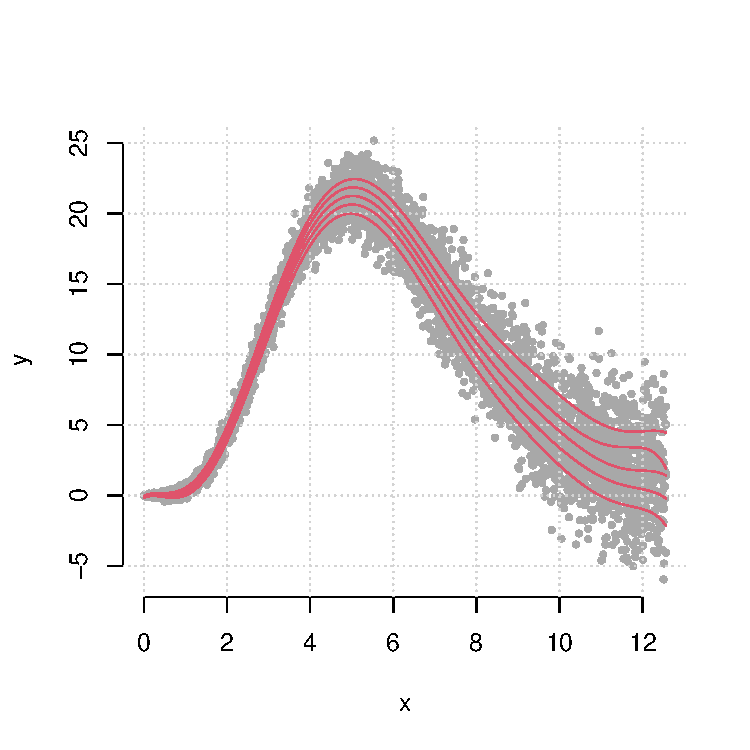
\includegraphics[width=.6\linewidth]{Figures/Uni02.pdf}
\caption{Example 1: fitted QR model for $q=1/6,2/6/3/6,4/6,5/6$}\label{Example1}
\end{figure} 
 
%\includeOutput{Univariate02}[tex]	


%\clearpage
\bibliographystyle{abbrvnat}
\begin{thebibliography}{99}
\bibitem{SEMMS}
{\rm Bar, H.~Y., Booth, J.~G., {\rm and} Wells, M.~T.} (2020).
\newblock {A Scalable Empirical Bayes Approach to Variable Selection in
  Generalized Linear Models}.
\newblock \emph{Journal of Computational and Graphical Statistics}, {\bf  0}\penalty0 (0), \penalty0 1--12.
\end{thebibliography}
\end{document}
